%%--SubSkipper Documentation
%%--Modified 25/07/15

\documentclass{article}

%%--packages
\usepackage{hyperref}
\usepackage{listings}
\usepackage{color}
\usepackage{graphicx}
\graphicspath{{figures/}}
\usepackage{geometry}

%%--Define Margins
 \geometry{
 a4paper,
 total={170mm,257mm},
 left=20mm,
 right=20mm,
 top=20mm,
 bottom=20mm,
 }


%%--Define style for Java code
\definecolor{dkgreen}{rgb}{0,0.6,0}
\definecolor{gray}{rgb}{0.5,0.5,0.5}
\definecolor{mauve}{rgb}{0.58,0,0.82}

\lstset{frame=tb,
  language=Java,
  aboveskip=3mm,
  belowskip=3mm,
  showstringspaces=false,
  columns=flexible,
  basicstyle={\small\ttfamily},
  numbers=none,
  numberstyle=\tiny\color{gray},
  keywordstyle=\color{blue},
  commentstyle=\color{dkgreen},
  stringstyle=\color{mauve},
  breaklines=true,
  breakatwhitespace=true,
  tabsize=3
}


%%--commands
\newcommand{\degree}{$^{\circ}$}

\author{Filip Socko}
\title{Fleet Boat Reference, Torpedo Solution Methods}

\begin{document}

\maketitle
\pagebreak
\tableofcontents
\pagebreak

\section{Introduction}
The GitHub SubSkipper repository contains the core logic of the app, such that it can be verified or used for other projects. This reference document contains the principles and equations on which the logic is based and some historical data.

The main purpose of the repository and documentation is to record techniques and methods of early submarine attack techniques in a way which are simple to employ in computer programs (i.e. showing mathematical equations where possible), as well as acting as a reference for Submarine Simulators.
\\ \\
This document is a reference for Torpedo types and common conversion factors, as well as types of US Fleet Boats and Types of US Torpedoes. A brief recognition manual will be provided in a separate document. This document also aims to provide a brief overview of common torpedo solution methods.

\section{Unit Conversions}

\subsection{Speed}
\begin{center}
\begin{tabular}{r | r}
$1.0$ knots & $1.0$ NM per hour\\
$1.0$ m/s & $1.94384449$ knots\\
$1.0$ m/s & $3.6$ km/h\\
\end{tabular}
\end{center}

\subsection{Length}
\begin{center}
\begin{tabular}{r | r}
$1.0$ NM & $1852.0$ m\\
$1.0$ km & $0.539956803$ NM\\
$1.0$ NM & $2025.37$ yards\\
$1.0$ NM & $6076.12$ feet\\
$1.0$ m & $3.2808399$ feet\\
$1.0$ m & $1.0936133$ yards\\
\end{tabular}
\end{center}

\section{Torpedo Data}

The following is torpedo for American torpedo types as used predominantly in the Pacific theatre.

Torpedo data adapted from \emph{SH4 V1.2 Ultimate Torpedo Guide} by Mechan, found at the ubisoft forums (http://forums.ubi.com/showthread.php/475595-SH4-V1-2-Ultimate-Torpedo-Guide-Forums). Dated: 06-22-2007, Accessed: 18.08.2015

Slow and Fast speeds and ranges removed as appropriate.

\subsubsection{Mark 10}
\begin{tabular}{l|l}
Available from:& Always\\
Range(m):& 3200\\
Speed(kt):&36\\
Warhead:& 80-160 radius 3-6m\\
Depth keeping:& 70\% chance of deviating $\pm 0.8m - \pm 1.2m$\\
Dud Chance (at AOB):& 1\% (0\degree -70\degree ) 25\% (70\degree-90\degree)\\
Renown cost:& 0\\
\end{tabular} \\
Notes: Default torpedo for the S-Class. Slower and with a shorter range than the Mk. 14, but extremely reliable.\\

\subsubsection{Mark 14}
\begin{tabular}{l|l}
Available from:& Always\\
Range(Slow)(m):& 8200\\
Range(Fast)(m):& 4100\\
Speed(Slow)(kt):&31\\
Speed(Fast)(kt):& 46\\
Warhead:& 100-170 radius 3-7m\\
Depth keeping:& 70\% chance of deviating $\pm 1.5m - \pm 3.3m$\\
Dud Chance (at AOB):& 1\% (0\degree-35\degree); 34\% (35\degree-70\degree); 99\% (70\degree-90\degree)\\
Renown cost:& 0\\
\end{tabular} \\
Notes: Default torpedo for all modern fleet boats. Faster and with a longer range than the Mk. 10, it packs a roughly 20\% stronger punch but is much less reliable.

\subsubsection{Mark 16}
\begin{tabular}{l|l}
Available from:& 1945-01-01\\
Range(m):& 12500\\
Speed(kt):&46\\
Warhead:& 180-250 radius 3.5-8m\\
Depth keeping:&  70\% chance of deviating $\pm 1.5m - \pm 3.3m$\\
Dud Chance (at AOB):& 4\% (0\degree-35\degree); 45\% (35\degree-70\degree); 100\% (70\degree-90\degree)\\
Renown cost:& 400\\
\end{tabular} \\
Notes: Fast torpedo with an exceptionally long range, but also terribly unreliable.

\subsubsection{Mark 18}
\begin{tabular}{l|l}
Available from:& 1943-07-12\\
Range(m):& 3650\\
Speed(kt):&29\\
Warhead:& 120-180 radius 3-7\\
Depth keeping fault chance:& 55\% chance of deviating $\pm 1.2m - \pm 2.8m$\\
Dud Chance (at AOB):& 1\% (0\degree-35\degree); 34\% (35\degree-70\degree); 99\% (70\degree-90\degree)\\
Renown cost:&  500 (200 from 1944-01-16; 0 from 1944-09-01)\\
\end{tabular} \\
Notes: Slower, 10\% more powerful, with a shorter range and much more reliable than the Mk. 14.

\subsubsection{Mark 23}
\begin{tabular}{l|l}
Available from:& 1943-01-01\\
Range(m):& 4100\\
Speed(kt):&46\\
Warhead:& 120-180 radius 3-7m\\
Depth keeping fault chance:& 70\% chance of deviating $\pm 1.5m - \pm 3.3m$\\
Dud Chance (at AOB):& 1\% (0\degree - 35\degree); 34\% (35\degree- 70\degree); 99\% (70\degree- 90\degree)\\
Renown cost:&  100 (0 from 16-01-1944)\\
\end{tabular} \\
Notes: Same range, speed and reliability than the Mk. 14 but roughly 10\% more powerful. Definitely replaces the Mk. 10 as the "standard" torpedo from 16-01-1944.

\subsubsection{Mark 27 "Cutie"}
\begin{tabular}{l|l}
Available From:& 1944-01-01\\
Range(m):& 4570\\
Speed(kt):&12\\
Warhead:& 50-100 radius 1.5-5\\
Depth keeping fault chance:& NA\\
Dud Chance (at AOB):& 1\% (0\degree-25\degree)\\
Renown cost:& 500\\
\end{tabular} \\
Notes: Slow acoustic homing torpedo with a small warhead primarily used for defence against destroyers.

\subsubsection{Torpedo minimum arming distance}
\emph{arming\_distance} is set across all torpedoes to 220m except the Mk. 27, which is 150 meters.
\subsubsection{Torpedo max dive angle}
\emph{max\_dive\_angle} is set to 20 degrees for all torpedo types.
\subsubsection{Torpedo maximum turn angle}
\emph{max\_turn\_angle} is 135\degree for all torpedoes except the Mk. 27, which is 180\degree.
\subsubsection{Magnetic detonation range}
\emph{mag\_detonation\_range} is 2m for all torpedoes except for the Mk. 27, which is 1m.
\subsubsection{Circular runner torpedos}
\emph{circle\_runner\_chance} is 0.5\% for all torpedoes except for the Mk. 27, which is 0\%.
\subsubsection{Gyro problems}
The chance of having gyro problems is 0.3\% at the introduction time of all torpedoes and drops to 0.2\% in later periods for all torpedoes except for the Mk. 16. The \emph{max\_deviation} when having gyro problems is always 50\degree. This does not apply to the Mk. 27. 
\subsubsection{Homing torpedos}
The Mk. 27 will run straight for 200m before homing.

\section{Trigger Maru Overhaul - Fleet Boat Types}
This section consists of pages 25-28 of the Trigger Maru Overhaul Manual which detail fleet boat types:
\includegraphics[page={25}, width=\textwidth, height=\textheight]{TMO_Manual}
\includegraphics[page={26}, width=\textwidth, height=\textheight]{TMO_Manual}
\includegraphics[page={27}, width=\textwidth, height=\textheight]{TMO_Manual}
\includegraphics[page={28}, width=\textwidth, height=\textheight]{TMO_Manual}

\section{Calculating AOB Based on Aspect Ratio}

Methods adapted from Angriffscheibe Handbuch by Karl Hahn, 2008.

AOB can be determined given the following data:
\begin{itemize}
%%\item{Range To Target} - Not sure
\item{Observed Mast Height}
\item{Observed Ship Length}
\item{Reference Aspect Ratio (i.e. $\frac{Reference Length}{Reference Mast Height}$)}
\end{itemize}

\subsubsection{Determine an observed \emph{aspect ratio}.}
$$AR\_{observed} = \frac{Observed Length}{Observed Mast Height}$$
As the required figure is a ratio, it does not matter in what units the figures are given. For example, this could be the number of degrees Length and Mast Heigh subtend, the number of periscope graduations subtended or angular length in metres. It only matters that units for Observed Mast Height and Observed Length are the same.

\subsubsection{Determine the Reference Apsect Ratio}
Identify the target and find the Length and Mast Height as given in the recognition manual (if possible) or calculate these figures using the SubSkipper ship parser. Proceed as for the observed aspect ratio to get the Reference Aspect Ratio (\emph{ARreference}).

\subsubsection{AOB calculation}
$$AOB = arcSin \frac{AR\_{observed}}{AR\_{reference}}$$

\begin{itemize}
\item{Note: This method is less accurate as AOB approaches 0. Indeed, using this method with a sample size of 16 at various AOBs, the average error was 9.1\degree and the median error 6.88\degree. The optimum range for collecting data seems to be around 2000m.}
\item{Note: This method does not compute whether the AOB is on the port or starboard side.}
\item{Note: "The AOB can only go up to 90, and gives no indication of starboard or port side showing. You have to determine that visually. If the target is moving away from you, you have to subtract the given angle from 180."\cite[p~15]{angrHandB, tvreAcqData} In Other words, the arcSin function has a domain of +90\degree to -90\degree. When the AOB is between 90\degree and 270\degree, subtract the result from 180\degree. \cite{arcSin}}

\item{AOB (Relative to Target) for each Quadrant:}
\begin{itemize}
	\item{0\degree - 90\degree : Use AOB result as is.}
	\item{90\degree - 180\degree : Subtract AOB result 				 from 180.}
	\item{180\degree - 270\degree : Subtract AOB result from 180, subtract result from 360.}
	\item{270\degree - 360\degree : Subtract AOB result from 360.}
	\end{itemize}

\end{itemize}


\section{Determine the distance to the track of a target}

As you manoeuvre into a firing position, it is useful to know your distance to the track of your target. Knowing the range and AOB of the target:

Track: intersection point between Submarine course and the current target course.

$$Distance to Track = Range \left( sin(AOB) \right)$$
%
%\section{Determine an optimum speed for attack position}
%
%To determine own speed needed to reach the target track in time to set up a torpedo solution. (Requires: Target Speed, Target AOB, Bearing to Target, Target Range, Distance to target track)
%
%\begin{enumerate}
%\item{Find distance T must travel to reach a bearing of 000\degree. If the track is known (see previous step) and bearing and range to target is known, time required is:
%$$ s = d/t  $$
%}

\section{O'Kane Torpedo Solution}
The Dick O'Kane method was devised by members of the Subsim.com\cite{subsim} forums. It is a constant bearing method which relies on calculating a lead angle -- an angle on which torpedoes, if launched will intercept the course of the target-- to which the periscope is pointed. As parts of the target ship cross the bearing, torpedoes are fired along it. The O'Kane method relies on being ahead of the target, and the final AOB -- at which the torpedo strikes the target-- to be 90\degree .

Calculates \emph{lead angle} based on target and torpedo speed.\\
The solution requires submarine to be ahead of target.\\
Captain inserts target speed into TDC, puts the scope on the lead bearing, fires as the target crosses the bearing.

The Equation for lead angle is as follows:

$$ LeadAngle = 90 - \arctan\left( \frac{Torpedo Speed}{TargetSpeed} \right) $$




\section{Determine the lead angle for a perpendicular attack with 0\degree gyro angle}

Once you are turned onto a perpendicular intercept course, this method calculates when to fire. The lead angle is simply the target bearing at the moment you fire. The range is irrelevant to the calculation although it is best to plan the attack within 500-1000m.

This is O'Kane, except more simple.

$$ lead angle = tan-1 ( [target speed / torpedo speed] ) $$


\section{Determine the torpedo gyro angle}
This example will show how to calculate the required gyro angle for a firing solution. This method is somewhat simplified and is best for smaller gyro angles (\textless 30\degree) and shorter ranges (\textless 1000 metres).

$$sin (lead angle) / sin (AOB) = (target speed) / (torpedo speed)$$
$$ gyroAngle = targetBearing -– leadAngle $$

%%TODO: shade alt rows

\pagebreak
\section{Knot to Km Travelled Conversion Chart}
\begin{table}[h]
\centering
\label{my-label}
\begin{tabular}{c|cccccccccc}
\textbf{Kt / Hr} & \textbf{1} & \textbf{2} & \textbf{3} & \textbf{4} & \textbf{5} & \textbf{6} & \textbf{7} & \textbf{8} & \textbf{9} & \textbf{10} \\
\hline
\textbf{1}       & 1.85       & 3.70       & 5.56       & 7.41       & 9.26       & 11.11      & 12.96      & 14.82      & 16.67      & 18.52       \\
\textbf{2}       & 3.70       & 7.41       & 11.11      & 14.82      & 18.52      & 22.22      & 25.93      & 29.63      & 33.34      & 37.04       \\
\textbf{3}       & 5.56       & 11.11      & 16.67      & 22.22      & 27.78      & 33.34      & 38.89      & 44.45      & 50.00      & 55.56       \\
\textbf{4}       & 7.41       & 14.82      & 22.22      & 29.63      & 37.04      & 44.45      & 51.86      & 59.26      & 66.67      & 74.08       \\
\textbf{5}       & 9.26       & 18.52      & 27.78      & 37.04      & 46.30      & 55.56      & 64.82      & 74.08      & 83.34      & 92.60       \\
\textbf{6}       & 11.11      & 22.22      & 33.34      & 44.45      & 55.56      & 66.67      & 77.78      & 88.90      & 100.01     & 111.12      \\
\textbf{7}       & 12.96      & 25.93      & 38.89      & 51.86      & 64.82      & 77.78      & 90.75      & 103.71     & 116.68     & 129.64      \\
\textbf{8}       & 14.82      & 29.63      & 44.45      & 59.26      & 74.08      & 88.90      & 103.71     & 118.53     & 133.34     & 148.16      \\
\textbf{9}       & 16.67      & 33.34      & 50.00      & 66.67      & 83.34      & 100.01     & 116.68     & 133.34     & 150.01     & 166.68      \\
\textbf{10}      & 18.52      & 37.04      & 55.56      & 74.08      & 92.60      & 111.12     & 129.64     & 148.16     & 166.68     & 185.20      \\
\textbf{11}      & 20.37      & 40.74      & 61.12      & 81.49      & 101.86     & 122.23     & 142.60     & 162.98     & 183.35     & 203.72      \\
\textbf{12}      & 22.22      & 44.45      & 66.67      & 88.90      & 111.12     & 133.34     & 155.57     & 177.79     & 200.02     & 222.24      \\
\textbf{13}      & 24.08      & 48.15      & 72.23      & 96.30      & 120.38     & 144.46     & 168.53     & 192.61     & 216.68     & 240.76      \\
\textbf{14}      & 25.93      & 51.86      & 77.78      & 103.71     & 129.64     & 155.57     & 181.50     & 207.42     & 233.35     & 259.28      \\
\textbf{15}      & 27.78      & 55.56      & 83.34      & 111.12     & 138.90     & 166.68     & 194.46     & 222.24     & 250.02     & 277.80      \\
\textbf{16}      & 29.63      & 59.26      & 88.90      & 118.53     & 148.16     & 177.79     & 207.42     & 237.06     & 266.69     & 296.32      \\
\textbf{17}      & 31.48      & 62.97      & 94.45      & 125.94     & 157.42     & 188.90     & 220.39     & 251.87     & 283.36     & 314.84      \\
\textbf{18}      & 33.34      & 66.67      & 100.01     & 133.34     & 166.68     & 200.02     & 233.35     & 266.69     & 300.02     & 333.36      \\
\textbf{19}      & 35.19      & 70.38      & 105.56     & 140.75     & 175.94     & 211.13     & 246.32     & 281.50     & 316.69     & 351.88      \\
\textbf{20}      & 37.04      & 74.08      & 111.12     & 148.16     & 185.20     & 222.24     & 259.28     & 296.32     & 333.36     & 370.40      \\
\textbf{21}      & 38.89      & 77.78      & 116.68     & 155.57     & 194.46     & 233.35     & 272.24     & 311.14     & 350.03     & 388.92      \\
\textbf{22}      & 40.74      & 81.49      & 122.23     & 162.98     & 203.72     & 244.46     & 285.21     & 325.95     & 366.70     & 407.44      \\
\textbf{23}      & 42.60      & 85.19      & 127.79     & 170.38     & 212.98     & 255.58     & 298.17     & 340.77     & 383.36     & 425.96      \\
\textbf{24}      & 44.45      & 88.90      & 133.34     & 177.79     & 222.24     & 266.69     & 311.14     & 355.58     & 400.03     & 444.48      \\
\textbf{25}      & 46.30      & 92.60      & 138.90     & 185.20     & 231.50     & 277.80     & 324.10     & 370.40     & 416.70     & 463.00      \\
\textbf{26}      & 48.15      & 96.30      & 144.46     & 192.61     & 240.76     & 288.91     & 337.06     & 385.22     & 433.37     & 481.52      \\
\textbf{27}      & 50.00      & 100.01     & 150.01     & 200.02     & 250.02     & 300.02     & 350.03     & 400.03     & 450.04     & 500.04      \\
\textbf{28}      & 51.86      & 103.71     & 155.57     & 207.42     & 259.28     & 311.14     & 362.99     & 414.85     & 466.70     & 518.56      \\
\textbf{29}      & 53.71      & 107.42     & 161.12     & 214.83     & 268.54     & 322.25     & 375.96     & 429.66     & 483.37     & 537.08      \\
\textbf{30}      & 55.56      & 111.12     & 166.68     & 222.24     & 277.80     & 333.36     & 388.92     & 444.48     & 500.04     & 555.60     
\end{tabular}
\end{table}

\section{Recognition Manual}


%%%END END END
\pagebreak
\begin{thebibliography}{9}

\bibitem{angrHandB}
  Karl Hahl,
  Kriegsmarine Angriffscheibe Handbuch,
  p. 15,
  2008.
  
\bibitem{tvreAcqData}
http://www.tvre.org/en/acquiring-torpedo-firing-data,
Acquiring torpedo firing data,
2015.

\bibitem{okane90Angles}
Corey "Gutted" Hardwell,
Silent Hunter IV 90\degree - AOB Firing Angles,
circ. 2008(?).

\bibitem{subsim}
http://www.subsim.com

\bibitem{arcSin}
MathOnWeb,
%http://mathonweb.com/help_ebook/html/functions_2.htm,
The arcsin function,
Accessed 17.08.2015,


\end{thebibliography}




\end{document}

